\documentclass[journal,12pt,twocolumn]{IEEEtran}

\usepackage{setspace}
\usepackage{gensymb}

\singlespacing


\usepackage[cmex10]{amsmath}

\usepackage{amsthm}

\usepackage{mathrsfs}
\usepackage{txfonts}
\usepackage{stfloats}
\usepackage{bm}
\usepackage{cite}
\usepackage{cases}
\usepackage{subfig}

\usepackage{longtable}
\usepackage{multirow}

\usepackage{enumitem}
\usepackage{mathtools}
\usepackage{steinmetz}
\usepackage{tikz}
\usepackage{circuitikz}
\usepackage{verbatim}
\usepackage{tfrupee}
\usepackage[breaklinks=true]{hyperref}
\usepackage{graphicx}
\usepackage{tkz-euclide}

\usetikzlibrary{calc,math}
\usepackage{listings}
    \usepackage{color}                                            %%
    \usepackage{array}                                            %%
    \usepackage{longtable}                                        %%
    \usepackage{calc}                                             %%
    \usepackage{multirow}                                         %%
    \usepackage{hhline}                                           %%
    \usepackage{ifthen}                                           %%
    \usepackage{lscape}     
\usepackage{multicol}
\usepackage{chngcntr}

\DeclareMathOperator*{\Res}{Res}

\renewcommand\thesection{\arabic{section}}
\renewcommand\thesubsection{\thesection.\arabic{subsection}}
\renewcommand\thesubsubsection{\thesubsection.\arabic{subsubsection}}

\renewcommand\thesectiondis{\arabic{section}}
\renewcommand\thesubsectiondis{\thesectiondis.\arabic{subsection}}
\renewcommand\thesubsubsectiondis{\thesubsectiondis.\arabic{subsubsection}}


\hyphenation{op-tical net-works semi-conduc-tor}
\def\inputGnumericTable{}                                 %%

\lstset{
%language=C,
frame=single, 
breaklines=true,
columns=fullflexible
}
\begin{document}


\newtheorem{theorem}{Theorem}[section]
\newtheorem{problem}{Problem}
\newtheorem{proposition}{Proposition}[section]
\newtheorem{lemma}{Lemma}[section]
\newtheorem{corollary}[theorem]{Corollary}
\newtheorem{example}{Example}[section]
\newtheorem{definition}[problem]{Definition}

\newcommand{\BEQA}{\begin{eqnarray}}
\newcommand{\EEQA}{\end{eqnarray}}
\newcommand{\define}{\stackrel{\triangle}{=}}
\bibliographystyle{IEEEtran}

\providecommand{\mbf}{\mathbf}
\providecommand{\pr}[1]{\ensuremath{\Pr\left(#1\right)}}
\providecommand{\qfunc}[1]{\ensuremath{Q\left(#1\right)}}
\providecommand{\sbrak}[1]{\ensuremath{{}\left[#1\right]}}
\providecommand{\lsbrak}[1]{\ensuremath{{}\left[#1\right.}}
\providecommand{\rsbrak}[1]{\ensuremath{{}\left.#1\right]}}
\providecommand{\brak}[1]{\ensuremath{\left(#1\right)}}
\providecommand{\lbrak}[1]{\ensuremath{\left(#1\right.}}
\providecommand{\rbrak}[1]{\ensuremath{\left.#1\right)}}
\providecommand{\cbrak}[1]{\ensuremath{\left\{#1\right\}}}
\providecommand{\lcbrak}[1]{\ensuremath{\left\{#1\right.}}
\providecommand{\rcbrak}[1]{\ensuremath{\left.#1\right\}}}
\theoremstyle{remark}
\newtheorem{rem}{Remark}
\newcommand{\sgn}{\mathop{\mathrm{sgn}}}
\providecommand{\abs}[1]{\left\vert#1\right\vert}
\providecommand{\res}[1]{\Res\displaylimits_{#1}} 
\providecommand{\norm}[1]{\left\lVert#1\right\rVert}
%\providecommand{\norm}[1]{\lVert#1\rVert}
\providecommand{\mtx}[1]{\mathbf{#1}}
\providecommand{\mean}[1]{E\left[ #1 \right]}
\providecommand{\fourier}{\overset{\mathcal{F}}{ \rightleftharpoons}}
%\providecommand{\hilbert}{\overset{\mathcal{H}}{ \rightleftharpoons}}
\providecommand{\system}{\overset{\mathcal{H}}{ \longleftrightarrow}}
	%\newcommand{\solution}[2]{\textbf{Solution:}{#1}}
\newcommand{\solution}{\noindent \textbf{Solution: }}
\newcommand{\cosec}{\,\text{cosec}\,}
\providecommand{\dec}[2]{\ensuremath{\overset{#1}{\underset{#2}{\gtrless}}}}
\newcommand{\myvec}[1]{\ensuremath{\begin{pmatrix}#1\end{pmatrix}}}
\newcommand{\mydet}[1]{\ensuremath{\begin{vmatrix}#1\end{vmatrix}}}

\numberwithin{equation}{subsection}

\makeatletter
\@addtoreset{figure}{problem}
\makeatother
\let\StandardTheFigure\thefigure
\let\vec\mathbf

\renewcommand{\thefigure}{\theproblem}

\def\putbox#1#2#3{\makebox[0in][l]{\makebox[#1][l]{}\raisebox{\baselineskip}[0in][0in]{\raisebox{#2}[0in][0in]{#3}}}}
     \def\rightbox#1{\makebox[0in][r]{#1}}
     \def\centbox#1{\makebox[0in]{#1}}
     \def\topbox#1{\raisebox{-\baselineskip}[0in][0in]{#1}}
     \def\midbox#1{\raisebox{-0.5\baselineskip}[0in][0in]{#1}}
\vspace{3cm}
\title{Assignment 4}
\author{KUSUMA PRIYA\\EE20MTECH11007}

\maketitle
\newpage

\bigskip
\renewcommand{\thefigure}{\theenumi}
\renewcommand{\thetable}{\theenumi}
Download all python codes from 
\begin{lstlisting}
https://github.com/KUSUMAPRIYAPULAVARTY/assignment4/tree/master/codes
\end{lstlisting}
%
and latex-tikz codes from 
%
\begin{lstlisting}
https://github.com/KUSUMAPRIYAPULAVARTY/assignment4
\end{lstlisting}
%
 
 \section{QUESTION}
Prove that the following equations represent two straight lines.Also find their point of intersection and the angle between them
\begin{align}
 3y^2-8xy-3x^2-29x+3y-18=0\label{1}
\end{align}

%

\section{Explanation}
The general form of equation representing a pair of straight lines is 
\begin{align}
    ax^2+2bxy+cy^2+2dx+2ey+f=0
\end{align}
This can be represented as
\begin{align}
    \vec{x}^T\vec{V}\vec{x}+2\vec{u}^T\vec{x}+f=0\\
    \text{where, } \vec{V}=\myvec{a&b\\b&c}\\ \vec{u}=\myvec{d\\e}
\end{align}
This represents a pair of straight lines if
\begin{align}
    \mydet{\vec{V}&\vec{u}\\\vec{u}^T&f}=0
\end{align}
\section{Solution}
\mydet{\vec{V}&\vec{u}\\\vec{u}^T&f} of \eqref{1} becomes
\begin{align}
    \mydet{-3&-4&-\frac{29}{2}\\-4&3&\frac{3}{2}\\-\frac{29}{2}&\frac{3}{2}&-18}\label{2}
\end{align}
Expanding equation \eqref{2}, we get zero.\\
Hence given equation represents a pair of straight lines.
\section{Finding the individual lines}
Slopes of the individual lines are roots of equation 
\begin{align}
    cm^2+2bm+a=0\\
    \implies 3m^2-8m-3=0\\
    \text{Solving, }m=3,-\frac{1}{3}
\end{align}
The normal vectors of the lines then become
\begin{align}
    \vec{n_1}=\myvec{\frac{1}{3}\\1}\\
    \vec{n_2}=\myvec{-3\\1}
\end{align}
Equations of the lines can therefore be written as
\begin{align}
  \myvec{\frac{1}{3}&1}\vec{x}=c\\
 \implies \myvec{1&3}\vec{x}=c_1 ,\\
   \myvec{-3&1}\vec{x}=c_2\\
  \implies \left[\myvec{1&3}\vec{x}-c_1\right]\left[\myvec{-3&1}\vec{x}-c_2\right]
\end{align}
represents the equation specified in \ref{?}\\
Comparing the equations, we have
\begin{align}
    \myvec{1&-3\\3&1}\myvec{c_2\\c_1}=\myvec{29\\-3}\\
 \end{align}
 Row reducing the augmented matrix
 \begin{align}
    \myvec{1&-3&29\\3&1&-3}\xleftrightarrow[]{R_2\leftarrow R_2-3\times R_1}
    \myvec{1&-3&29\\0&10&-90}\\
    \xleftrightarrow[]{R_2\leftarrow R_2\times \frac{1}{10}}
    \myvec{1&-3&29\\0&1&-9}\\
    \xleftrightarrow[]{R_1\leftarrow R_1+3\times R_2}
    \myvec{1&0&2\\0&1&-9}\\
    \implies c_2=2 \text{ and }c_1=-9
\end{align}
The individual line equations therefore become
\begin{align}
    \myvec{1&3}\vec{x}=-9\label{3} ,\\\myvec{-3&1}\vec{x}=2\label{4}
\end{align}
Note that the convolution of the normal vectors, should satisfy the below condition
\begin{align}
    \myvec{1\\3}*\myvec{-3\\1}=\myvec{a\\2b\\c}\label{5}
\end{align}
The LHS part of \eqref{5} can be rewritten using toeplitz matrix as
\begin{align}
    \myvec{1&0\\3&1\\0&3}\myvec{-3\\1}=\myvec{-3\\-8\\3}=\myvec{a\\2b\\c}
\end{align}
\section{Intersection Point}
The augmented matrix for the set of equations represented in \eqref{3}, \eqref{4} is
\begin{align}
\myvec{1&3&-9\\-3&1&2}
\end{align}
Row reducing the matrix
\begin{align}
 \myvec{1&3&-9\\-3&1&2}\xleftrightarrow[]{R_2\leftarrow R_2+3\times R_1}\myvec{1&3&-9\\0&10&-25}\\
 \xleftrightarrow[]{R_1\leftarrow R_1-\frac{3}{10}\times R_2}\myvec{1&0&-\frac{3}{2}\\0&10&-25}\\
 \xleftrightarrow[]{R_2\leftarrow \frac{R_2}{10}}\myvec{1&0&-\frac{3}{2}\\0&1&-\frac{5}{2}}\\
\text{Hence, the intersection point is}
\myvec{-\frac{3}{2}\\-\frac{5}{2}}
\end{align}
\begin{figure}[!ht]
\centering
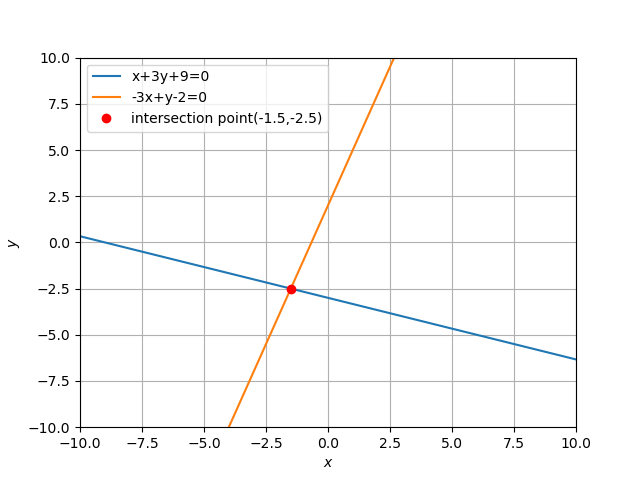
\includegraphics[width=\columnwidth]{hw4plot.png}
\caption{plot showing intersection of lines}
\label{Fig}
\end{figure}
\newpage
\section{Angle Between The Lines}
Angle between two lines $\theta$ can be given by
\begin{align}
\cos \theta = \frac{\vec{n_1}^T\vec{n_2}}{\norm{\vec{n_1}}\norm{\vec{n_2}}}
\end{align}
From \eqref{3}, \eqref{4},
\begin{align}
\cos \theta=\frac{\myvec{1&3}\myvec{-3\\1}}{\sqrt{(3)^2 +1} \times \sqrt{(-3)^2 +1}}=0\\
\implies \theta = 90\degree
\end{align}
\end{document}

